\section{Типы планет. Формирование планетных систем.}
\subsection{Классификация по составу}
\begin{wrapfigure}{r}{0.5\textwidth}
  \begin{center}
    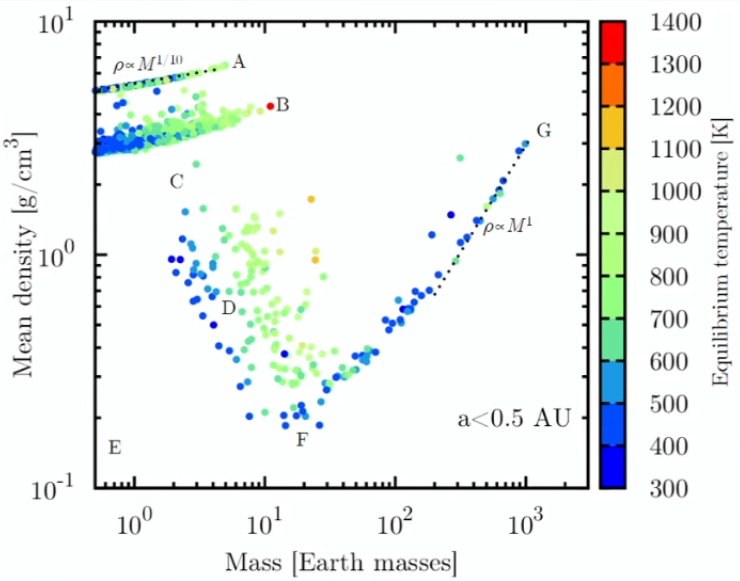
\includegraphics[width=0.48\textwidth]{Pictures/4_types.png}
  \end{center}
  \caption{График зависимости плотности планеты от ее массы: результаты моделирования. Цвет характеризует температуру планеты.}
  \label{fig:4_types}
\end{wrapfigure}
Основная классификация качественно представлена на графике \ref{fig:4_types}: 

A -- Твердые каменные. Плотность растет с увеличением массы, но очень медленно.

B -- Твердые ледяные. Плотность тоже растет медленно.

C -- Испаряющиеся.

D -- Маломассивные планеты с большими ядрами, тем не менее, обладающие толстой атмосферой, состоящая из легких элементов (водород и/или гелий). Такой состав атмосферы является причиной низкой средней плотности, при расчете которого учитывается \textit{видимый} радиус планеты.

E -- Запрещенная зона.

F -- Переход к планетам- гигантам.

G -- Планеты - гиганты. Газовые, следовательно, более сжимаемые объекты $\implies$ плотность растет быстро с ростом массы. 

\subsection{Основные типы планет}

\begin{wrapfigure}{l}{0.65\textwidth}
  \begin{center}
    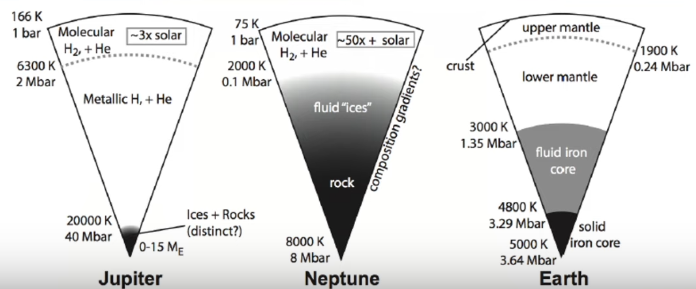
\includegraphics[width=0.63\textwidth]{Pictures/4_solar_types.png}
  \end{center}
  \caption{Типы планет}
  \label{fig:4_solar_types}
\end{wrapfigure}

Определяются \textit{основной} компонентой состава (рис.\ref{fig:4_solar_types}):

\paragraph{Газовые гиганты}: \textbf{H/He} (почти звездный состав). Планеты-гиганты, масса от 0.19 до 13 масс Юпитера. \textbf{Быстро вращаются.} Из-за колоссального давления в недрах планеты водород переходит в металлическую фазу (становится вырожденным). Радиус планет близок к радиусу \textbf{Юпитера}, или примерно в 10-11 раз превышает радиус Земли. Исключение составляют т.н. "горячие юпитеры" - планеты-гиганты, расположенные близко к своей звезде и имеющие эффективную температуру выше $1000\,\text{K}$. Сильно нагретая светом близкой звезды, их атмосфера расширяется, увеличивая видимый радиус планеты до 1-1.4 радиуса Юпитера. Средняя плотность гигантов меняется от 0.28 г/куб.см (самые разреженные горячие юпитеры) до 12 г/куб.см (самые массивные планеты-гиганты в 10-12 масс Юпитера). Скорее всего, все планеты-гиганты имеют сильное магнитное поле, усиливающееся с ростом массы планеты.

В Солнечной системе планеты-гиганты - Юпитер и Сатурн. 


\paragraph{Ледяные гиганты}: \textbf{H/He+лед+ядро. Нептуны}, масса от 7 до 60 масс Земли. Состоят большей частью из льдов (водяного, аммиачного, метанового, сероводородного) и скальных пород, составляющих примерно четверть полной массы планеты. Доля водорода и гелия в составе планеты не превышает 15-20$\%$. Давление в недрах недостаточно для перехода водорода в металлическую фазу. Радиус близок к 4 радиусам Земли. Средняя плотность составляет 1.3-2.2 г/куб.см. Магнитное поле сильно отличается от дипольного (например, планета может иметь два северных и два южных полюса).

В Солнечной системе нептуны - Уран и Нептун. 

\paragraph{Твердые планеты} \textbf{Si, Mg, Fe, C, O}. Железно-каменные планеты, планеты \textbf{земного типа}, масса меньше 7 масс Земли. Состоят в основном из силикатов и железа. Средняя плотность 3.5-6 г/куб.см. Радиус меньше 2 радиусов Земли.

В Солнечной системе планеты земного типа - Меркурий, Венера, Земля и Марс. 

\subsection{Формирование планетных систем}

\begin{wrapfigure}{r}{0.48\textwidth}
  \begin{center}
    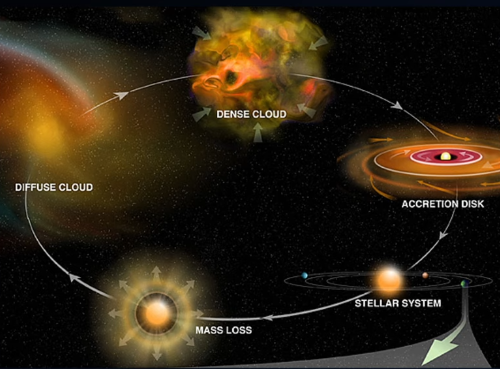
\includegraphics[width=0.5\textwidth]{Pictures/4_spiral.png}
  \end{center}
  \caption{Галактический спиралеворот: Формирование и распад планетной системы}
  \label{fig:4_spiral}
\end{wrapfigure}Существует много способов формирования планет. Основным путем образования планет считается путь снизу вверх (от мелких объектов к планетам).

Вокруг звезды, возникает протопланетный диск из смеси газа (которого много) и пыли (ее мало). Состав и свойства диска определяются межзвездной средой. В результате слияний, пылевые частицы начинают расти, вырастают в более крупные объекты. Если вокруг много газа, то эти объекты начинают его притягивать. Большие планеты растут из-за аккреции газа, а маленькие планеты растут слабо только за счет поглощения твердых объектов. Вблизи солнца образуются маленькие каменные планеты, потому что тяжелых элементов мало, а дальше, где газа много, образуются газовые гиганты. Большие планеты всегда обязаны быть газовыми, потому что только водорода и гелия много. Вблизи звезды начинает плавиться пыль ($\ge 1300\,\text{K}$), но при удалении от звезды температура падает (по закону Стефана-Больцмана). 

\paragraph{Снеговая линия} Многие газы могут замерзать, образовывая ледяные пылинки. Снеговая линия -- критическое расстояние от звезды, на котором температура достаточно низкая для этого процесса, соответственно, внутри снеговой линии не могут существовать и расти ледяные тела. Для Солнца она находится примерно на расстоянии 3 а.е.

Достаточно тяжелые ледяные объекты, начинают корректировать газ и возникает ледяной гигант. 
\newpage
\subsubsection{Миграция планет}

\begin{wrapfigure}[17]{l}{0.3\textwidth}
  \begin{center}
    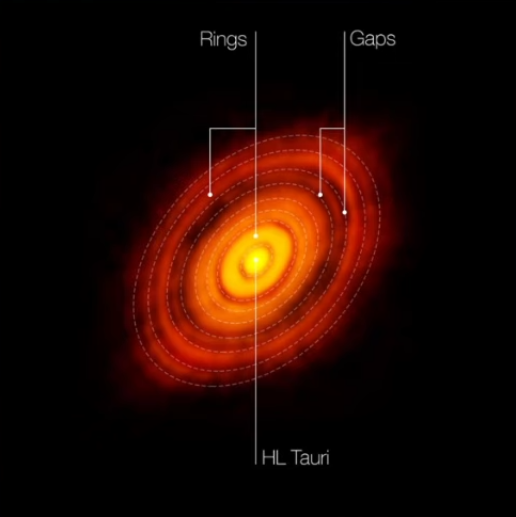
\includegraphics[width=0.28\textwidth]{Pictures/4_disk_gaps.png}
  \end{center}
  \caption{Протопланетный диск HL Тельца}
  \label{fig:4_disk}
\end{wrapfigure}Планета не сохраняется на одном радиусе, мигрируя преимущественно внутрь системы из-за взаимодействия с веществом диска и ''расталкивая'' его. 
При взаимодействии с частицей с меньшим радиусом орбиты, планета притягивает и тормозит ее, уменьшая ее полную энергию. Следовательно, частица переходит на \textit{более низкую} орбиту. Аналогично планета отталкивает частицы, находящиеся снаружи своей орбиты.

Однако не все планеты создают такую щель, как на \mbox{рисунке \ref{fig:4_disk}}. Если планета не достигла критической массы, взаимодействие будет слабым и вещество будет ''протекать''. Если же планета открывает щель, ее миграция замедляется.

Однако, создав щель, планета не перестает расти. Таким образом, планета служит мостом для передачи вещества и углового момента, ''протекающих'' через нее.(рис. \ref{fig:4_brige})
Миграция оказывает влияние на вид системы и может значительно поменять ее вид. 
\begin{wrapfigure}[23]{r}{0.4\linewidth}
  \begin{center}
    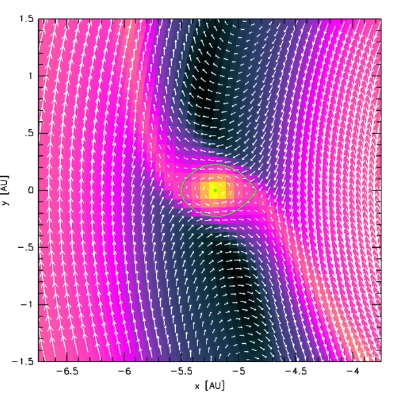
\includegraphics[width=\linewidth]{Pictures/4_brige.png}
  \end{center}
  \caption{''Мост''}
  \label{fig:4_brige}
\end{wrapfigure}
Причина, по которой планетные системы выглядят сжатыми (вся ''жизнь'' происходит в одном месте, близко к звезде по сравнению с размерами системы), заключается во взаимодействии планет при миграции. Миграция массивных внешних планет сдвигает более мелкие, внутренние планеты к центру системы.

С течением времени планета становится все массивнее, и влияние на диск -- заметнее.

\paragraph{Фанфакты}

\begin{itemize}

    \item \textbf{Эффект Лидова-Козаи} В системе трёх тел у орбиты может меняться одновременно и эксцентиситет, и наклон. Этим объясняется движение планет в системе в противоположные стороны (изначально все планеты находятся в одной плоскости и движутся в одном направлении).  
    \item \textbf{Приливы} Если планета находится блико к звезде, она будет возбуждать прилив, который будет приводить к торможению планеты, сл, переход на более низку орбиту, и, в конечном счете, разрушение/поглощение звездой. Событие редкое. Еще планета может испариться/перетечь в звезду.

    \item \textbf{Цикличность} Процесс образования новых звезд планетных систем идет непрерывно, как и выброс вещества в межзвездную среду (\mbox{рис. \ref{fig:4_spiral}}). На каждом последующем цикле появляется больше тяжелых элементов (первые звезды не могли иметь каменные планеты).
    
    \item \textbf{Фрагментация диска} Крупные планеты могут образовываться на больших расстояниях (за снеговой линией, 10 а.е и больше) от звезды как результат неустойчивости диска: гравитационно связанные объекты сжимяется и мигрирует, преврящаясь в планету в бурые карлики. Ситуация редкая ($\sim$ 1$\%$ планет)
    
\end{itemize}
